\documentclass[12pt]{article}
\usepackage[ngerman]{babel}
\usepackage{amsmath}
\usepackage[utf8]{inputenc}
\usepackage{hyperref}
\usepackage{algorithm,algpseudocode}
\usepackage{setspace}
\setstretch{1.5}
\usepackage[paper=a4paper,left=25mm,right=35mm,top=25mm,bottom=20mm]{geometry}
\usepackage{graphicx}
\usepackage{wrapfig}

\hypersetup{
    colorlinks,
    citecolor=black,
    filecolor=black,
    linkcolor=black,
    urlcolor=black
}

\begin{document}

\renewcommand{\figurename}{Abb.}
\def\figureautorefname{Abb.}
\def\algorithmautorefname{Alg.}

\floatname{algorithm}{Alg.}

\title{Extremwertproblem Wegfindung \\  \large{\enspace Vergleich verschiedener Algorithmen}}

\author{Maximilian Stark}

\maketitle
\thispagestyle{empty}
\clearpage

\tableofcontents
\thispagestyle{empty}
\clearpage

\section{Einleitung}
\newpage

\section{Grundlagen und Terminologie}
\label{sec:basics}
Zu Beginn werden in diesem Abschnitt die grundlegenden Begriffe der Graphen-Theorie geklärt. Auch Fachbegriffe aus der Implementierung durch die Informatik werden erläutert.
\\
Das Ziel dieser Arbeit ist die Darstellung und der Vergleich verschiedener \textit{Wegfindungs-Algorithmen} in der Anwendung an verschiedenen generierten \textit{Graphen}.
\\
Zugrunde all dem liegt die Graphen-Theorie. Deren Fundament ist der namensgebende \textit{Graph} $G\; = \{V,\,E\}$, alternativ auch \textit{Netz} genannt, welcher aus einer Menge von \textit{Knoten} $V$ 
(von engl. "`Vertex") und aus einer Menge \textit{Kanten} $E$ (von engl. "`Edge").
\\
Zeichnerisch werden \textit{Knoten} als Punkte oder Kreise dargestellt; \textit{Kanten} als Verbindungslinien zwischen zwei \textit{Knoten}. Jede \textit{Kante} hat einen \textit{Startknoten} und
einen \textit{Endknoten}. Wenn von einer \textit{gerichteten Kante} die Rede ist, lässt sich das als Pfeil interpretieren, da die Verbindung unidirektional gilt. Ebenso gibt es die \textit{gewichteten Kanten}, 
denen nicht nur zwei \textit{Knoten} zugeordnet werden, sondern zusätzlich noch ein Gewicht $w$ (von engl. "`Weight"), ein Zahlenwert, der als Kosten der Beziehung zwischen den beiden \textit{Knoten} gesehen werden kann.
\\
In der Wegfindung ist ein \textit{Weg} $P$ (von engl. "`Path") als geordnete Abfolge von \textit{Knoten} definiert. Da in der Regel jedes \textit{Knoten}-Paar nur einfach verbunden ist, reicht in der Implementierung 
dieser Ansatz aus.
\\
Visuell wird der \textit{Graph} durch einen \textit{Layout-Algorithmus} dargestellt, welcher allen \textit{Knoten} durch gewisse Berechnungen Positionen zuteilt (vgl. \autoref{sec:layout}).
\\
Generell sind \textit{Algorithmen} eine festgelegte Abfolge von Schritten um Daten zu verarbeiten. In der Informatik sind diese einzelnen Schritte Befehle.
\\
Um ein \textit{Netz} zu generieren, wird eine Zufallsfunktion verwendet. Hierzu wird ein standardisierter \textit{Pseodozufall}-Generator verwendet \cite{random}. Dieser generiert kaum oder nur schwer vorhersagbare Abfolgen 
von Zahlen und genügt für unsere Zwecke. Aufgrund der nicht echten Zufälligkeit wird ein sogenanntes \textit{Seed}-System benutzt, eine spezielle Zahl, mit deren Übergabe an den Generator stets die selbe Zahlenfolge erzeugt
werden kann.
\newpage
\section{Aufbau und Bedienung des Programms}
\label{sec:manual}
Das Programm, im eigentlichen Fokus stehend, fungiert sowohl als visuelle Möglichkeit der Darstellung, als auch als Quelle für Vergleichsdaten und Messungen in selbst erzeugten Szenarien.
Geschrieben ist das Programm in der Programmiersprache \textit{Java} unter Verwendung der \textit{JavaFX}-Standardbibliothek \cite{javafx}.
\begin{figure}[h!]
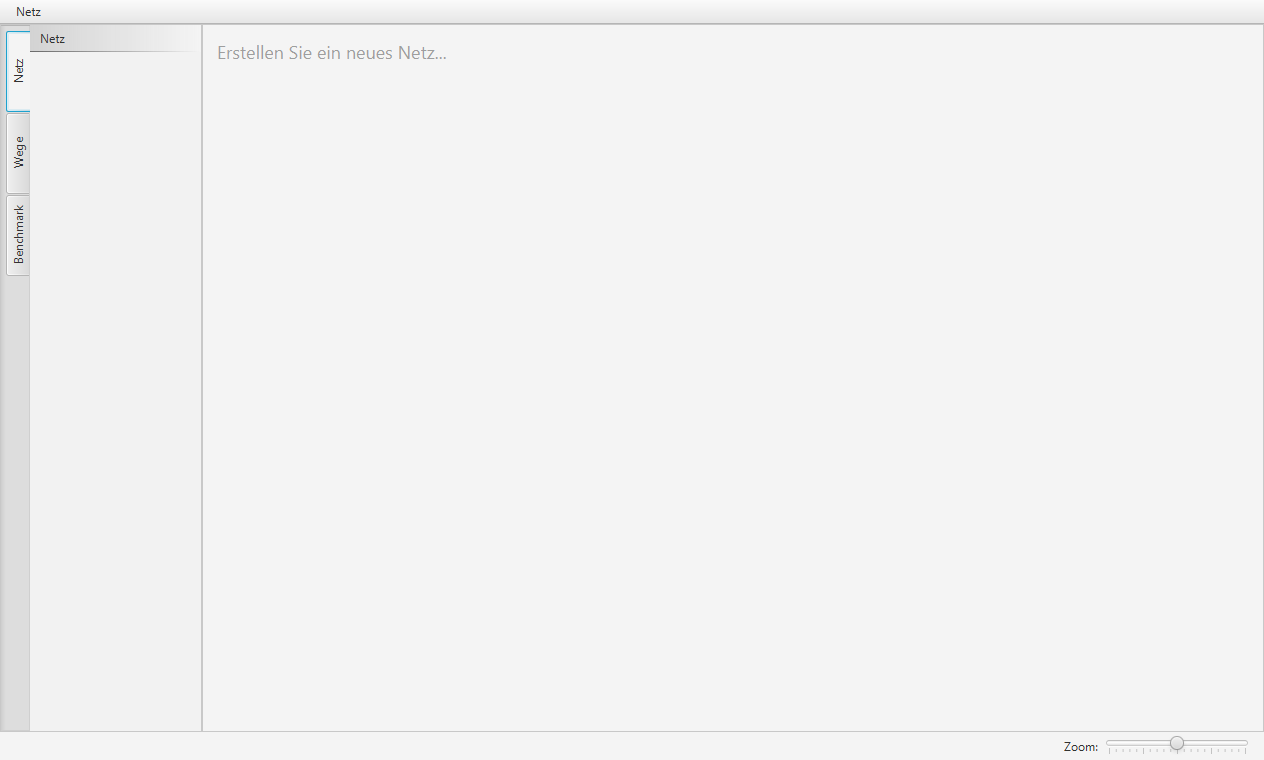
\includegraphics[width=0.8\textwidth]{res/main_screenshot.png}
\centering
\caption{Die Start- und Hauptansicht der Applikation}
\label{fig:main_screenshot}
\end{figure}
\\
Auf den ersten Blick ist die Anwendungsoberfläche in zwei größere Bereiche aufgeteilt. Im linken, kleineren Seitenbereich werden detaillierte Informationen über den \textit{Graphen}, bereits berechnete \textit{Wege} und 
die Konfigurationsmöglichkeiten neuer Wege, in mehreren "`Tabs" unterteilt, angezeigt. Der große rechte Bereich, zu Beginn der Anwendung nur mit "`Erstellen Sie ein neues Netz..." (\autoref{fig:main_screenshot}) 
beschriftet, dient als Hauptansicht von sowohl des \textit{Graphen}, als auch der Vergleichsstatistiken und Tabellen.
\\
Die Bedienung kann vollständig mit der Maus erfolgen, da sich sämtliche Features visuell intuitiv und minimalistisch präsentieren. Nur vereinzelt führen Tastatureingaben oder "`Hotkeys"\;zu mehr Komfort oder Genauigkeit 
der Anwendung. So kann beispielsweise das \textit{Relayout} (siehe \autoref{sec:layout}) des \textit{Graphen} per "`L"\;Taste, das \textit{Generieren} (siehe \autoref{sec:construct}) eines neuen unter Benutzung 
von "`N".
\\
\newpage
\section{Konstruktion des Graphen}
\label{sec:construct}
Im nächsten Schritt werden wir nun einen Graphen erzeugen lassen und die Funktionsweise des Generators betrachten. 
Durch Klicken auf "`Erstellen Sie ein neues Netz..."\;wird ein Dialog-Fenster geöffnet (\autoref{fig:new_graph_screenshot}), welches verschiedene 
\begin{wrapfigure}{l}{0.5\textwidth}
\vspace{-20pt}
\begin{center}
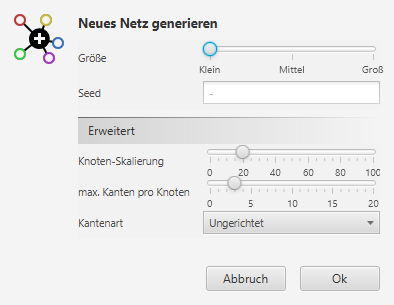
\includegraphics[scale=0.6]{res/new_graph_screenshot.png}
\end{center}
\vspace{-20pt}
\centering
\caption{Dialog zur \textit{Netz}-Generierung}
\label{fig:new_graph_screenshot}
\end{wrapfigure}
Genererierungs-\textit{Parameter} zur Konfiguration anbietet. 
\\
Unterteilt sind diese Einstellungen in zwei Bereiche: \textit{Generell} und \textit{Erweitert}. \textit{Generelle} Optionen sind für den einfachen Gebrauch ausreichend mit einem Regler für die Größe $s$ und einem 
\textit{Seed}\footnote{\hyperref[sec:basics]{Abschnitt \ref*{sec:basics} - \nameref{sec:basics}}}-Eingabefeld ausgestattet.
\\
Im \textit{Erweitert}-Bereich lässt sich die Generierung aufs Genaueste einstellen. So können die Anzahl an Maximalknoten $n_{max}$ und die maximale \textit{Kanten}-Anzahl $e_{max}$ pro \textit{Knoten} 
festgelegt werden. Ebenso kann die Wahl zwischen drei Typen $t$ von \textit{Kanten} getroffen werden: \textit{Ungerichtet}, \textit{Gemischt} und \textit{Gerichtet}\footnotemark[1], was alle \textit{Kanten} des zu 
generierenden \textit{Graphen} betrifft. Die Option \textit{Gemischt} bewirkt, dass die Gerichtetheit jeder \textit{Kante} zufallsbedingt ist.
\\
Durch Bestätigen per Klick auf "`Ok" wird der Generator mit diesen \textit{Parametern} gestartet.
\\
Zunächst wird der \textit{Seed} für den Zufallsgenerator gesetzt. Danach wird aus den gegebenen Grenzwerten die tatsächliche Menge von \textit{Knoten} berechnet und in den \textit{Graphen} eingesetzt. Daraufhin wird für jeden 
\textit{Knoten} eine Anzahl an \textit{Kanten} bestimmt. Durch das "`Clampen", d.h Einzwicken, Eingrenzen, der Start- und 
Generierungswerte durch
\vspace{-20pt}
\begin{gather*}
e = max(1,\,R(0,\;min(n/2-1,\,e_{max}))) \\
\left(\begin{aligned}
max(a, b) \to \text{Größere der beiden Parameter}\\
min(a, b) \to \text{Kleinere der beiden Parameter}
\end{aligned}
\right)
\end{gather*}
wird gewährleistet, dass der Generator nicht mehr \textit{Kanten} platzieren kann, als eindeutig möglich ist. Jetzt wird versucht, sämtliche \textit{Knoten} durch zufällige Wahl mit einem anderen 
\textit{Knoten} zu verbinden, wobei der jeweils gesuchte \textit{Knoten} weder der Ausgangsknoten selbst, noch ein bereits verbundener \textit{Knoten} sein soll. Sobald eine Kombination gefunden wurde, 
wird die entsprechende \textit{Kante} mit einem ebenfalls zufallsgenerierten \textit{Gewicht} erstellt. Dann wird auf Basis des \textit{Kanten-Typs} die Gerichtetheit bestimmt und schließlich wird die 
\textit{Kante} im \textit{Graphen} platziert (\autoref{alg:generatorv2}).

\begin{algorithm}
\caption{\textit{Graph-Generator v1} \label{alg:generator}}
\begin{algorithmic}[1]
\Statex
\Require {Zufallsgenerator R, max. Kantengewicht $W_{max} = 30$}
\Ensure {Graph g}
\Statex
\Procedure{generateGraph}{$seed$, s, $n_{max}$, $e_{max}$, $t$}
	\State $R.seed \gets seed$
	\State $n \gets (R(0,\,n_{max}/2) + n_{max}/2) * s$
	\State add \textit{n} nodes to \textit{g}
	\For {$i=0 \to n$}
		\State $e \gets max(1,\,R(0,\;min(n/2-1,\,e_{max})))$
		\For {$j=0 \to e$}
			\State $index \gets i$
			\Repeat 
				\State $index \gets R(0,\,n)$
			\Until $index = i \text{ or \textit{g.nodes}[\textit{i}] is connected to \textit{g.nodes}[\textit{index}]}$
			
			\State $e \gets \text{edge from \textit{g.nodes}[\textit{i}] to \textit{g.nodes}[\textit{index}], } w = R(0, W_{max})$
			\If {$t = 1 \text{ or } (t = 2 \text{ and } R() > R())$}
				\State $e.directed \gets true$
			\EndIf
			\State add \textit{e} to \textit{g}
		\EndFor
	\EndFor
\EndProcedure

\end{algorithmic}
\end{algorithm}

% damit die erste fassung komplett auf english bleibt erst hier 
\renewcommand{\algorithmicrequire}{\textbf{geg.:}}
\renewcommand{\algorithmicensure}{\textbf{ges.:}}
\renewcommand{\algorithmicprocedure}{\textbf{prozedur}}
\renewcommand{\algorithmicfor}{\textbf{für}}
\renewcommand{\algorithmicdo}{\textbf{wiederhole}}
\renewcommand{\algorithmicend}{\textbf{ende}}
\renewcommand{\algorithmicrepeat}{\textbf{wiederhole}}
\renewcommand{\algorithmicif}{\textbf{wenn}}
\renewcommand{\algorithmicthen}{\textbf{dann}}
\renewcommand{\algorithmicuntil}{\textbf{solange}} % for the classic do ... while
\newcommand{\sei}{\textbf{sei }}

\begin{algorithm}
\caption{\textit{Graph-Generator v2} \label{alg:generatorv2}}
\begin{algorithmic}[1]
\Statex
\Require {Zufallsgenerator R, max. Kantengewicht $W_{max} = 30$}
\Ensure {Graph g}
\Statex
\Procedure{generiereGraph}{$seed$, $s$, $n_{max}$, $e_{max}$, $t$}
	\State setze Seed von $R$ zu $seed$
	\State \sei $n$ $R(n_{max}/2,\,n_{max}) * s$ \Comment Zufällige Anzahl im Interval $\big[n_{max}/2;\;n_{max}\big[$
	\State füge $n$ $Knoten$ zu $g$ hinzu
	\For {$i=0 \to n$}
		\State \sei $e$ $max(1,\,R(0,\;min(n/2-1,\,e_{max})))$
		\For {$j=0 \to e$}
			\State \sei $index$ $i$
			\Repeat 
			\State \sei $index$ $R(0,\,n)$
			\Until $index$ gleich $i$ oder $Knoten_{i}$ mit $Knoten_{index}$ verbunden
			\State \sei $e$ Kante von $Knoten_{i}$ zu $Knoten_{index}$, Gewicht $w = R(0, W_{max})$
			\If {$t =$ \textsc{Gemischt} oder $(t =$ \textsc{Gerichtet} und $R() > R())$} \State \Comment $R>R =$ Zufallstest
				\State setze $e$ gerichtet
			\EndIf
			\State füge $e$ zu $g$ hinzu
		\EndFor
	\EndFor
\EndProcedure
\end{algorithmic}
\end{algorithm}

\clearpage
\section{Visuelles Layout des Graphen}
\label{sec:layout}
In vorangegangen Abschnitten wurde das grundlegende Konzept eines \textit{Graphen} bereits dargestellt. Wenn man sich nun Gedanken dazu macht, wie denn ein solch abstraktes Konstrukt optimal visuell zu präsentieren ist,
begibt man sich in die Thematik des \textit{Layouts} (von engl. "`Anordnung") eines \textit{Graphen}.
\newpage

\section{Wegfindungs-Algorithmen}
\newpage

\subsection{Gröbste Züge von Intelligenz: Tiefensuche}
\newpage
-
\newpage

\subsection{Heuristik als Mittel zum Ziel: Der Dijkstra-Algorithmus}
\newpage
-
\newpage

\subsection{Der Allstar: Der A*-Algorithmus}
\newpage
-
\newpage

\section{Vergleichsstatistik und Fazit}
\newpage
-
\newpage

\section{Schluss}
\newpage

\begin{thebibliography}{9}
\bibitem{random} Java Zufalls-Funktion http://docs.oracle.com/javase/7/docs/api/java/util/Random.html \emph{abgerufen am 18.10.15}
\bibitem{javafx} JavaFX-Homepage http://docs.oracle.com/javase/8/javafx/get-started-tutorial/jfx-overview.htm \emph{abgerufen am 14.10.15}
\end{thebibliography}

\end{document}
